\documentclass[10pt]{article}
\usepackage[utf8]{inputenc}
\usepackage[T1]{fontenc}
\usepackage{lmodern}
\usepackage[margin=0.8in,columnsep=0.3in]{geometry}
\usepackage{tikz}
\usetikzlibrary{arrows.meta,decorations.pathreplacing}
\usepackage{booktabs}
\usepackage{xcolor}
\usepackage[hidelinks]{hyperref}
\usepackage{float}

\setlength{\parindent}{0pt}
\setlength{\parskip}{0.4em}

\definecolor{barsolid}{RGB}{25,25,25}
\definecolor{bargray}{RGB}{143,143,137}
\definecolor{nbblue}{RGB}{21,87,166}
\definecolor{nbred}{RGB}{190,60,70}

\newcommand{\sweepSmall}{\draw[line width=1.2pt,color=barsolid] (0,10) -- (1,9) -- (2,10) -- (3,9) -- (4,2) -- (5,2);\fill[barsolid] (0,10) circle (2.4pt);\fill[barsolid] (1,9) circle (2.4pt);\fill[barsolid] (2,10) circle (2.4pt);\fill[barsolid] (3,9) circle (2.4pt);\fill[barsolid] (4,2) circle (2.4pt);\fill[barsolid] (5,2) circle (2.4pt);}
\newcommand{\sweepBig}{\draw[line width=1.2pt,color=nbblue] (0,10) -- (1,10) -- (2,10) -- (3,10) -- (4,10) -- (5,10);\fill[nbblue] (0,10) circle (2.4pt);\fill[nbblue] (1,10) circle (2.4pt);\fill[nbblue] (2,10) circle (2.4pt);\fill[nbblue] (3,10) circle (2.4pt);\fill[nbblue] (4,10) circle (2.4pt);\fill[nbblue] (5,10) circle (2.4pt);}
\newcommand{\fieldtable}{\begin{table}[H]\centering\footnotesize\setlength{\tabcolsep}{3.5pt}\begin{tabular}{@{}llrrrr@{}}\toprule Window & Sampling & Tools & Tokens in & Correct & 95\% CI \\\midrule
4,096 & default & 24 & 2,050 & 0/10 & 0--31\% \\
4,096 & low temp. & 24 & 2,050 & 0/10 & 0--31\% \\
4,096 & default & 1 & 1,317 & 10/10 & 69--100\% \\
4,096 & low temp. & 1 & 1,317 & 10/10 & 69--100\% \\
\midrule
32,768 & default & 24 & 14,095 & 10/10 & 69--100\% \\
32,768 & low temp. & 24 & 14,095 & 9/10 & 55--100\% \\
32,768 & default & 1 & 1,317 & 10/10 & 69--100\% \\
32,768 & low temp. & 1 & 1,317 & 10/10 & 69--100\% \\
\bottomrule\end{tabular}\caption{Same model, same request, two server windows. “Correct call” = a call to the right tool with the right command.}\label{tab:field}\end{table}}
\newcommand{\controltable}{\begin{table}[H]\centering\footnotesize\setlength{\tabcolsep}{3.5pt}\begin{tabular}{@{}rrrrrr@{}}\toprule Tools & Tokens & A, 4,096 & B, 4,096 & A, 32,768 & B, 32,768 \\\midrule
4 & 1,566 & 10/10 & 10/10 & 10/10 & 10/10 \\
8 & 3,243 & 10/10 & 10/10 & 10/10 & 10/10 \\
16 & 6,594 & 0/10 & 0/10 & 10/10 & 10/10 \\
24 & 9,943 & 0/10 & 0/10 & 10/10 & 10/10 \\
\bottomrule\end{tabular}\caption{Synthetic control at equal total tokens. A: $k$ tools. B: one tool, system prompt padded to the same size as A. Correct calls out of 10.}\label{tab:control}\end{table}}


\title{\LARGE\bfseries The Cliff Was the Context Window\\[2pt]\large\mdseries A silent prompt truncation that looked like a tool-count limit}
\author{
  {\large Ricardo Martínez}\\[2pt]
  {\small Cloud Security \& Applied AI}
}
\date{\small November 2026}

\begin{document}
\twocolumn[
  \begin{@twocolumnfalse}
    \maketitle
    \begin{abstract}
    \noindent
    A 9.7B open-weight model behind a local inference server passed a one-tool smoke test and then never called a single tool once it was connected to an agent with 24 tool schemas. Sweeping the number of tools made it look like a cliff between 8 and 16 tools. It was not. The agent's request weighed 14,095 tokens, the server's default window was 4,096, and the server cut the prompt to about 2,050 tokens without telling the client, dropping the front of the prompt, where the tool schemas sit. The request had asked for a 262,144-token window through an option the OpenAI-compatible endpoint did not honor. With the window raised to 32,768, the same request produced a correct call in 10 of 10 trials at default sampling, and the sweep was flat at 10 of 10 from 1 to 24 tools. Lowering the sampling temperature changed nothing in either window. A synthetic control confirms it: one tool with the prompt padded to the size of 24 tools fails, and succeeds, exactly where the 24-tool request does. Before concluding that a small model cannot use tools, read the effective context.
    \end{abstract}
    \vspace{1.2em}
  \end{@twocolumnfalse}
]

\section{What happened}

An open-weight model (Qwen3.5 9B, Q4\_K\_M, 9.7B parameters) served by Ollama 0.33.2 on one machine with 17.8 GiB of VRAM was wired into an open-source agent framework through the OpenAI-compatible endpoint. Asked to run a script, the agent answered in prose: it wrote the command in a code block and described what it would do, without calling the terminal tool that was in its payload. A direct one-tool test with the same model passed.

Three explanations were plausible. The model is too small for tool use. The sampling defaults (temperature 1, presence penalty 1.5) make it improvise. Or 24 tools are too many for it. A variant with temperature 0.1 and no presence penalty did not change the agent's behavior.

\section{Capturing the request}

We pointed the framework at a local proxy that records each request body and answers with fixed text, so nothing was executed. The request carried 24 tool schemas, an 18,536-character system prompt, a 20-token user message and \texttt{options.num\_ctx = 262144}. Counted on a server whose window is large enough to avoid truncation, it weighed 14,095 tokens: 9,686 for the tools, 4,372 for the agent's instructions, 20 for the message and 17 of chat template (Figure~\ref{fig:bar}).

\begin{figure}[H]
\centering
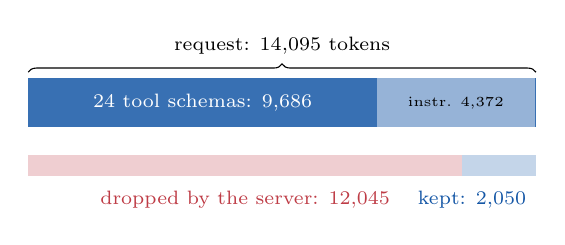
\begin{tikzpicture}[x=0.00046cm,y=1cm]
\def\h{0.62}
\fill[nbblue!85] (0,0) rectangle (9686,\h);
\fill[nbblue!45] (9686,0) rectangle (14058,\h);
\fill[nbblue!85] (14058,0) rectangle (14095,\h);
\fill[nbred!25] (0,-0.62) rectangle (12045,-0.35);
\fill[nbblue!25] (12045,-0.62) rectangle (14095,-0.35);
\node[font=\scriptsize,text=white] at (4843,\h/2) {24 tool schemas: 9,686};
\node[font=\tiny] at (11872,\h/2) {instr. 4,372};
\node[font=\scriptsize,text=nbred,anchor=north] at (6022,-0.68) {dropped by the server: 12,045};
\node[font=\scriptsize,text=nbblue,anchor=north east] at (14095,-0.68) {kept: 2,050};
\draw[decorate,decoration={brace,amplitude=3pt}] (0,\h+0.08) -- (14095,\h+0.08) node[midway,above=3pt,font=\scriptsize] {request: 14,095 tokens};
\end{tikzpicture}
\caption{The captured request at the default window of 4,096 tokens (to scale). The server keeps the first few tokens and the tail, and the tool schemas sit at the front.}
\label{fig:bar}
\end{figure}

\section{Replaying it}

We replayed the captured request against the same model, ten trials per condition (Table~\ref{tab:field}).

\fieldtable

At the server's default window of 4,096 tokens the model made no correct call in 20 of 20 trials, under default and low-temperature sampling. At 32,768 it made one in 10 of 10 and 9 of 10 (the one miss called a different tool). The one-tool request passed in all four conditions, including default sampling, so the earlier impression that lowering the temperature rescued it did not reproduce under repeated trials.

The server explains the difference. At 4,096 it logged \texttt{truncating input prompt} with a limit of 2,050 for a 14,095-token prompt, 50 times during the run, and none at 32,768. The response carried no error, and its usage field reported 2,050 prompt tokens.

A probe shows what survived. At 4,096, asked to repeat two markers placed at the start and at the end of the system message, the model reported not seeing the first and read the second; asked to list its tools, it listed skill names that live in the system prompt, not the functions. At 32,768 it read both markers and listed all 24 function names. The model's chat template appears to place the tool block before the system text (we did not print the rendered prompt), which fits the probe: the cut removes the beginning, so the schemas go first.

\section{It looks like a tool-count cliff}

Figure~\ref{fig:sweep} sweeps the number of tools with a short system prompt, using subsets of the 24 real schemas.

\begin{figure}[H]
\centering
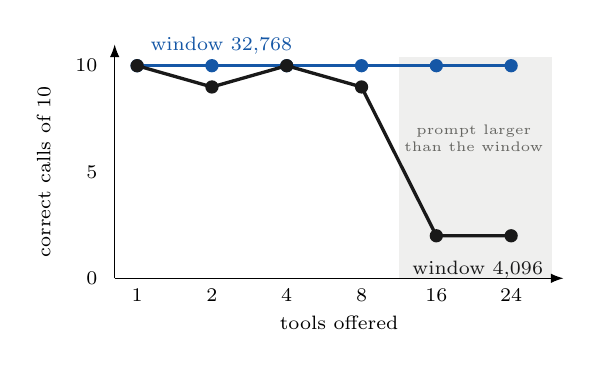
\begin{tikzpicture}[x=0.95cm,y=0.27cm]
\fill[bargray!14] (3.5,0) rectangle (5.55,10.4);
\node[font=\tiny,text=bargray!70!black,align=center] at (4.5,6.6) {prompt larger\\than the window};
\draw[-{Latex[length=1.6mm]},line width=0.4pt] (-0.3,0) -- (5.7,0);
\draw[-{Latex[length=1.6mm]},line width=0.4pt] (-0.3,0) -- (-0.3,11);
\foreach \i/\k in {0/1,1/2,2/4,3/8,4/16,5/24} {\node[font=\scriptsize] at (\i,-0.8) {\k};}
\foreach \y in {0,5,10} {\node[font=\scriptsize,anchor=east] at (-0.4,\y) {\y};}
\node[font=\scriptsize] at (2.7,-2.1) {tools offered};
\node[font=\scriptsize,rotate=90] at (-1.25,5) {correct calls of 10};
\sweepBig
\sweepSmall
\node[font=\scriptsize,text=nbblue,anchor=west] at (0.05,10.95) {window 32,768};
\node[font=\scriptsize,text=barsolid,anchor=north west] at (3.55,1.25) {window 4,096};
\end{tikzpicture}
\caption{Correct calls out of 10 at each tool count, same model, same subsets, same prompts. Only the server window changes. At 4,096 the curve falls between 8 and 16 tools, where the prompt starts to exceed the window; at 32,768 it is flat.}
\label{fig:sweep}
\end{figure}

A reader who stopped at the dark curve would have reported a tool-count cliff. The blue curve is the same experiment with one setting changed.

\section{Control: tools versus size}

The sweep above changes the tool count and the prompt size together. To separate them, a public harness with no private data builds synthetic tools of realistic size (about 420 tokens each) and compares two arms at the same total number of tokens. Arm A offers $k$ tools with a short system prompt. Arm B offers one tool and pads the system prompt with neutral text up to the size of arm A (Table~\ref{tab:control}).

At 4,096 the two arms behave the same: 10 of 10 while the prompt fits (up to 3,243 tokens) and 0 of 10 once it does not (6,594 and 9,943 tokens, clipped to 2,050). In those failing cells the model wrote the command as text in 34 of 40 trials and made a tool call in only 2 of 40, neither correct. At 32,768 all cells are 10 of 10. One tool is as vulnerable as 24 once the prompt outgrows the window, and 24 tools are as safe as one while it does not. What matters is the size of the prompt against the window; the tools only matter by being large.

\controltable

\section{Mechanism and fix}

Ollama's documentation gives default context lengths by VRAM (4k below 24 GiB) and states that the OpenAI API has no way of setting the context size for a model, so it recommends a Modelfile with \texttt{PARAMETER num\_ctx} \cite{ollama-ctx,ollama-openai}. Our server logged a 4,096 window for a request that carried \texttt{num\_ctx = 262144} in \texttt{options}. A Modelfile variant with \texttt{num\_ctx 32768} on an otherwise default server returned a correct call in 5 of 5 trials with no truncation warnings. The documentation recommends at least 64,000 tokens for agents; this payload alone takes 14,095 before any conversation.

\section{What to check first}

\begin{itemize}
\item Compare \texttt{usage.prompt\_tokens} in the response with what you sent. At 4,096 the server reported 2,050 for a 14,095-token request and raised no error.
\item Search the server log for \texttt{truncating input prompt}, and read the \texttt{CONTEXT} column of \texttt{ollama ps}.
\item When going through \texttt{/v1}, set the window in the model (Modelfile), not in request options.
\item Certify tool use with the production payload, not with the smoke test. A pass at one tool is evidence about one tool.
\end{itemize}

\section{Related work}

Tool-count degradation is documented. In LangChain's ReAct benchmark, GPT-4o fell to 2\% on calendar scheduling at seven domains and Llama-3.3-70B failed to call a required tool in every case \cite{langchain}. Maxim AI reports that cutting a GitHub and Notion toolset from 48 to 25 tools improved four of five models, with Claude Sonnet 4 moving from 66.67\% to 73.33\% \cite{maxim}. Anthropic reports Claude Opus 4.5 moving from 79.5\% to 88.1\% on an internal MCP evaluation when tools are discovered on demand, a vendor figure \cite{anthropic}. A May 2026 preprint reports Phi-4 14B restored from 0\% to 84.4\% at 20 tools by compiling schemas, on the author's own benchmark \cite{tscg}. Those studies measure selection under growing context. Our case is a different mechanism: the tools never reached the model. We did not check whether any cited run suffered truncation; reporting the effective window would let readers tell.

\section*{Limits}

One model (Qwen3.5 9B, Q4\_K\_M), one server version (Ollama 0.33.2), one machine, one task (run one shell command), ten trials per cell. In the control, the padding precedes the instruction and we did not test padding after it; the synthetic tools are generic and the target tool sits at two thirds of the list. With ten trials, 0 of 10 and 10 of 10 are separable (exact 95\% intervals 0--31\% and 69--100\%), small differences are not. Reasoning effort was medium, as in the captured request. We did not record the original server configuration on the day of the failure: the replay reproduces the same prose answers at the default window, which is consistent with, but does not prove, that the original runs were truncated the same way. The two Ollama pages disagree on the default (VRAM-dependent versus 4,096); our server logged 4,096 at 17.8 GiB. An earlier version of this repository called this a tool-count cliff and a categorical collapse of small models. That claim was wrong, and these measurements replace it.

{\small\setlength{\itemsep}{0pt}\begin{thebibliography}{9}
\bibitem{langchain} LangChain. \textit{Benchmarking Single Agent Performance}. February 10, 2025. blog.langchain.com/react-agent-benchmarking.
\bibitem{maxim} Maxim AI. \textit{How We're Measuring Model-Tool Accuracy in the Age of MCP}. July 2025. getmaxim.ai/blog.
\bibitem{anthropic} Anthropic. \textit{Introducing advanced tool use on the Claude Developer Platform}. November 24, 2025. anthropic.com/engineering/advanced-tool-use.
\bibitem{tscg} F. Sakizli. \textit{TSCG: Deterministic Tool-Schema Compilation for Agentic LLM Deployments}. arXiv:2605.04107, May 2026.
\bibitem{ollama-ctx} Ollama. \textit{Context length}. docs.ollama.com/context-length.
\bibitem{ollama-openai} Ollama. \textit{OpenAI compatibility}. docs.ollama.com/api/openai-compatibility.
\end{thebibliography}}

\end{document}
